\documentclass[14pt]{article}
\usepackage{float}
\usepackage
[
        a4paper,% other options: a3paper, a5paper, etc
        left=2cm,
        right=2cm,
        top=3cm,
        bottom=4cm,
]
{geometry}

\usepackage[utf8]{inputenc}
\usepackage{listings}
\usepackage{xcolor}
\usepackage{graphicx}
\lstset { %
    language=C++,
    backgroundcolor=\color{black!5}, % set backgroundcolor
    basicstyle=\footnotesize,% basic font setting
}


\title{Report.4.threads}
\author{lehuyduc3 }
\date{November 2020}
\usepackage{indentfirst}
\parindent{}

\begin{document}

\maketitle

\section{How to implement labwork}
We use a loop to test the dimension of the blocks: 8x8 to 32x32.
For the grid dim, we use enough blocks so that each pixel is processed by exactly 1 thread.
For each number of thread, we create enough block so that each pixel is processed by exactly 1 thread.

The kernel is as follow:
\begin{lstlisting}
__global__
void rgb2gray_labwork4(char* goutput, char* ginput, int height, int width, int pixelCount)
{
	const int row = blockIdx.x * blockDim.x + threadIdx.x,
			  col = blockIdx.y * blockDim.y + threadIdx.y;
	
	if (row < height && col < width) {
		const int i = row * width + col;
		goutput[i * 3] = (char)((int(ginput[i * 3]) + int(ginput[i * 3 + 1]) + int(ginput[i * 3 + 2])) / 3);
        goutput[i * 3 + 1] = goutput[i * 3];
        goutput[i * 3 + 2] = goutput[i * 3];
	}			  
}
\end{lstlisting}

The launch configuration is as follow:
\begin{lstlisting}
dim3 gridDim = dim3(height / blockSize + 1, width / blockSize + 1, 1);
dim3 blockDim = dim3(blockSize, blockSize, 1);
rgb2gray_labwork4<<<gridDim, blockDim>>>(goutput, ginput, height, width, pixelCount);
\end{lstlisting}

\section{Execution time and speedup}

\begin{figure}[H]
\centering
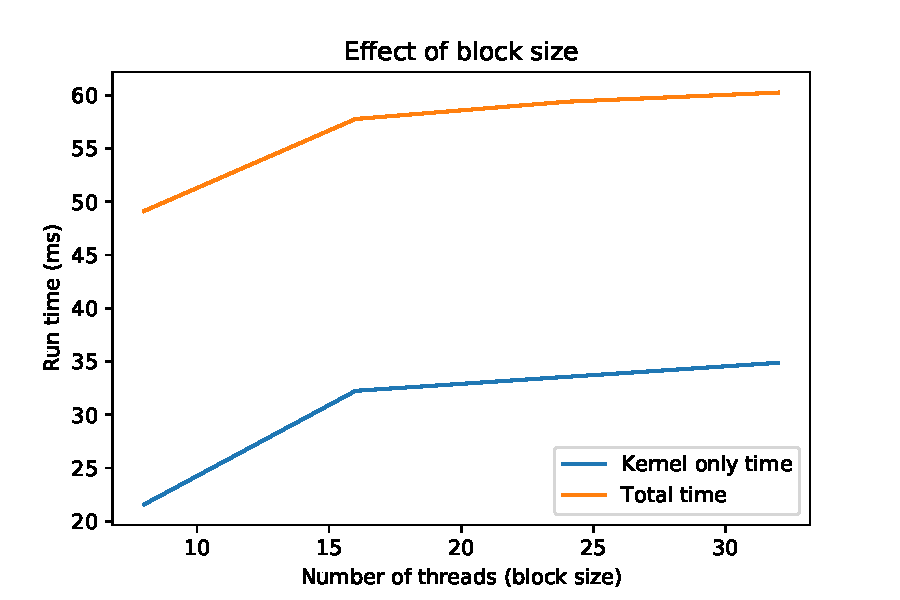
\includegraphics{report4_runtime.pdf}
\end{figure}

We see that performance actually decreases when block size is bigger. This is due to more overhead.

From the previous report, we know that performance is best when number of threads per block is 64. Since the $rgb2grayscale$ has mostly memory access and very little computation, more threads (block size = 16 means 256 threads per block) does not give better result.

\end{document}
